\index{regression function}
\index{generalization}

\subsection*{Introduction}

Here the neural network learns from knowledge represented by a data set consisting of input-target instances. The targets
are a specification of what the response to the inputs should be, and are represented as continuous variables. 

The basic goal in a function regression problem is to model the
conditional distribution of the target variables, conditioned on
the input variables \cite{Bishop1995}. This function is called the
regression function.

The formulation of a function regression problem requires:

\begin{itemize}
\item[-] A data set. 
\item[-] A neural network.
\item[-] A performance functional.
\item[-] A training strategy.
\item[-] A model selection algorithm.
\item[-] A testing method.
\end{itemize}

A common feature of most data sets is that the data
exhibits an underlying systematic aspect, represented by some
function, but is corrupted with random noise. 

The central goal is to produce a model which exhibits good generalization, or in other words, one which makes good predictions for new data. The best generalization to new data is obtained when the mapping represents the underlying
systematic aspects of the data, rather capturing the specific
details (i.e. the noise contribution) of the particular input-target
set. 

\subsection*{Data set}

\index{data set}
\index{training data set}
\index{generalization data set}
\index{testing data set}

Table \ref{DataSetFunctionRegressionTable} shows the format of a data set for function regression. 
It consists $q$ instances consisting of $n$ input variables and $m$ target variables. 
All input and targets are real values. 

\begin{table}[h!]
\begin{center}
\begin{tabular}{|ccc|ccc|}
\hline
$input_{1,1}$ & $\ldots$ & $input_{1,n}$ & $target_{1,1}$ & $\ldots$ & $target_{1,m}$\\
$input_{2,1}$ & $\ldots$ & $input_{2,n}$ & $target_{2,1}$ & $\ldots$ & $target_{2,m}$\\
$\vdots$ &  & $\vdots$ & $\vdots$ &  & $\vdots$\\ 
$input_{q,1}$ & $\ldots$ & $input_{q,n}$ & $target_{q,1}$ & $\ldots$ & $target_{q,m}$\\
\hline
\end{tabular}\caption{Data set for function regression.}
\label{DataSetFunctionRegressionTable}
\end{center}
\end{table}

When solving function regression problems it is always convenient to split the data set into a training, a generalization and a testing subsets. The size of each subset is up to the designer. Some default values could be to use $60\%$, $20\%$ and $20\%$ of the instances for training, generalization and testing, respectively. 

There are several data splitting methods. Two common approaches are to generate random indices or to specify the required indices for the training, generalization and testing instances.

A simple statistical analysis must be always performed in order to chech for data consistency. Basic statistics of a data set include the mean, standard deviation, minimum and maximum values of input and target variables for the whole data set and the training, generalization and testing subsets. An histogram of each input and target variables should also be plot in order to check the distribution of the available data. 

Also, it is a must to scale the data with the data statistics. 
There are two main data scaling methods, the mean and standard deviation and the minimum and maximum. 

The mean and standard deviation method scales the data for mean $0$ and standard deviation $1$. 
The minimum and maximum method scales the data for minimum $-1$ and maximum $1$. 

\subsection*{Neural network}
\index{neural network}

A neural network is used to represent the regression function. 
The number of inputs must be equal to the number of inputs in the data set, $n$, and the number of outputs must be the number of targets, $m$. 
This neural network will contain a scaling layer, a multilayer perceptron and an unscaling layer. 
It might optionally contain a bounding layer. 
Figure \ref{NeuralNetworkFunctionRegressionFigure} shows a general neural network for solving function regression problems. 

\begin{figure}[h!]
\begin{center}
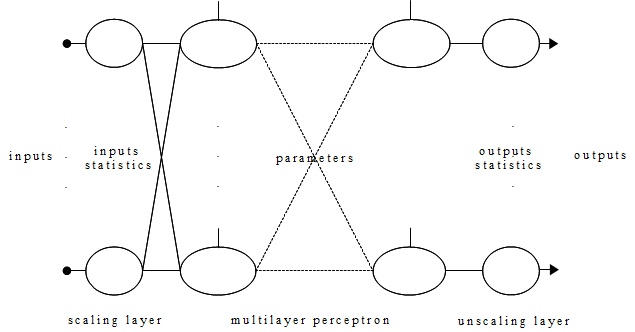
\includegraphics[width=1.2\textwidth]{function_regression/neural_network_function_regression.png}
\caption{Neural network for function regression.}\label{NeuralNetworkFunctionRegressionFigure}
\end{center}
\end{figure}

In general, using a multilayer perceptron with a one hidden layer will be enough. 
A default value to start with for the size of that layer could be 

\begin{eqnarray}\nonumber
\text{hidden neurons number}=\frac{\text{inputs number + outputs number}}{2}. 
\end{eqnarray}

Please note that the complexity which is needed depends very much on the problem at hand, and the above equation is just a rule of thumb. 
However, there are standard methods to find the correct complexity of a neural network for function regression problems. 
The most common is called model selection, which is described later in this section.  

The activation functions for the hidden layers and the output layer are also design variables. 
However, hyperbolic tangent activation function for the hidden layers and linear activation function for the output layer are widely used when solving function regression problems. 

Scaling of inputs and unscaling of outputs should not be used in the design phase, since the data set has been scaled already. When moving to a production phase, the inputs scaling and outputs unscaling methods should be coherent with the scaling method used for the data. 

The neural network in Figure \ref{NeuralNetworkFunctionRegressionFigure} spans a parameterized function space. 
That parameterized space of functions will be the basis to aproximate the regression function. 

\subsection*{Performance functional}
\index{performance functional, function regression}
\index{error functional}

The regression function can be evaluated quantitatively by means of a performance functional of the form

\begin{eqnarray}\nonumber
\text{Performance functional = objective term + regularization term}. 
\end{eqnarray}

For function regression problems, the objective term is measures the error between the outputs from the neural network and the targets in the data set.

In function regression problems, regularization is normally used when the number of instances in the data set 
is small or when the data is noisy. In other situations, regularization might not be necessary.    
  
The solution approach to a function regression problem for is to obtain a neural network which minimizes the performance functional. 
Note that neural networks represent functions. 
In that way, the function regression problem is formulated as a variational problem.


\subsection*{Training strategy}
\index{training algorithm, function regression}

The training strategy is entrusted to solve the reduced function optimization problem by minimizing the performance function. 

In general, evaluation, gradient and Hessian of the error function can be computed analytically. 
Zero order training algorithms, such as the evolutionary algorithm, converge extremely slowly and they are not a good choice. 

On the other hand, second order training algorithms, such as the Newton's method, need evaluation of the Hessian and are neither a good choice. 

In practice, first order algorithms are recommended for solving function regression problems. The Levenberg-Marquardt is a good choice for small and medium sized problems. Due to storage requirements, that algorithm is not recommended for big sized problems, and a quasi-Newton method with BFGS training direction and Brent training rate is preferable. 

In order to study the convergence of the optimization process, it is useful to plot the behaviour of some variables related to the multilayer perceptron, the error functional or the training algorithm as a function of the iteration step. 
Some common training history variables are: 

\begin{itemize}
\item[-] Parameters norm history. 
\item[-] Evaluation history. 
\item[-] Generalization evaluation history. 
\item[-] Gradient norm history. 
\item[-] Training direction norm history. 
\item[-] Training rate history. 
\item[-] Elapsed time history.
\end{itemize}

Form all the training history variables, may be the most important one is the evaluation history. 
Also, it is important to analyze the final values of some variables. 
The most important training results numbers are: 

\begin{itemize}
\item[-] Final parameters. 
\item[-] Final parameters norm. 
\item[-] Final error. 
\item[-] Final generalization error. 
\item[-] Final gradient. 
\item[-] Final gradient norm. 
\item[-] Number of iterations. 
\item[-] Training time. 
\end{itemize}

\subsection*{Model selection}
\index{model selection}

Two frequent problems in function regression are called underfitting and overfitting. 
The best generalization is achieved by using a model whose complexity is the most appropriate to produce an adequate fit of the data \cite{Bishop1995}. 
In this way underfitting is defined as the effect of a generalization error increasing due to a too simple model, 
whereas overfitting is defined as the effect of a generalization error increasing due to a too complex model.

%Figure XXX shows an underfitting case for a function regression problem. 
%In this case we have used a neural network which is too simple to produce an adequate fit. 

%Figure XXX. Underfitting illustration.

%Figure XXX shows an overfitting case for a function regression problem. 
%Here the error on the training data set is very small, but when new data is presented to the neural network the error is large. The neural network has memorized the training examples, but it has not learned to generalize to new situations. 
%The model is too complex to produce an adequate fit.
%Figure XXX. Overfitting illustration.

%Finally, Figure XXX shows a case in which the neural network has a proper complexity to produce a good fit of the data.
%Figure XXX. Good fitting illustration.

While underfitting can be prevented by simply increasing the complexity of the neural network, it is more difficult in advance to prevent overfitting.

A common method for preventing overfitting is to use a regularization term in the performance functional expression. 

However, the best method for avoiding underfitting and overfitting is to use a neural network that is just large enough to provide an adequate fit. 
Such a neural network will not have enough power to overfit the data. 
Unfortunately, it is difficult to know beforehand how large a neural network should be for a specific application.
A technique for that is called model selection. 

In this technique the data set is divided into a training and a generalization subsets. 
The training subset is used for training the neural network by means of the training strategy. 
On the other hand, the error on the generalization subset is monitored during the training process. 
The generalization error normally decreases during the initial phase of training, as it does the training error.

However, when the neural network begins to overfit the data, the error on the generalization subset typically begins to rise. 
When the generalization error increases for a specified number of iterations, the training is stopped, and the parameters at the minimum of the generalization error are set to the neural network.

This process is repeated for several network architectures, and the final training and generalization errors are plotted. 
The optimal network architecture will be that providing minimal generalization error. 
Figure \ref{ModelSelectionFunctionRegression} illustrates this generalization analysis. 

\begin{figure}[h!]
\begin{center}
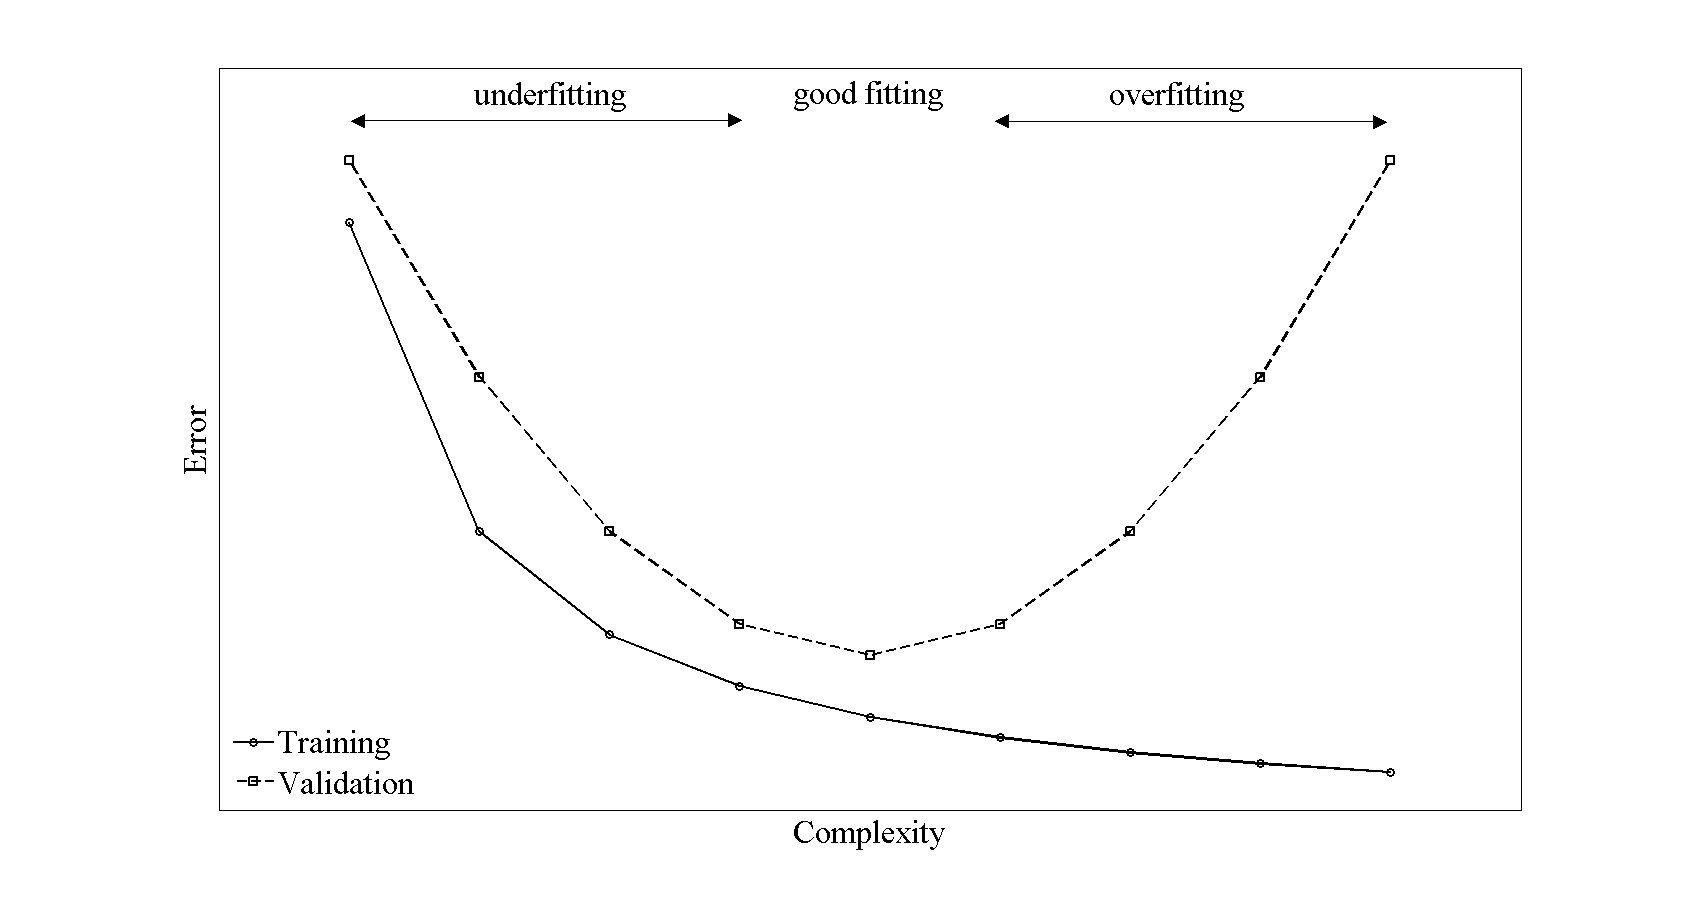
\includegraphics[width=1.0\textwidth]{function_regression/model_selection.png}
\caption{Model selection plot for function regression.}\label{ModelSelectionFunctionRegression}
\end{center}
\end{figure}


\subsection*{Testing analysis}
\index{linear regression analysis}

The performance of a neural network can be measured to some extent
by the performance evaluation on the testing set, but it is useful to
investigate the response in more detail. One option is to perform
a regression analysis between the network response and the
corresponding targets for an independent testing subset.

This analysis leads to $3$ parameters for each output variable. The first two parameters, $a$ and $b$,
correspond to the y-intercept and the slope of the best linear
regression relating outputs and targets. The third parameter, $R^{2}$,  is the correlation coefficient between the outputs and the targets. 

If we had a perfect fit (outputs exactly equal to targets), the slope would be $1$, and the
y-intercept would be $0$. If the correlation coefficient is equal to $1$, then there is perfect correlation between
the outputs from the neural network and the targets in the testing subset. 

Figure \ref{LinearRegressionAnalysis} illustrates a linear regression analysis.  

\begin{figure}[h!]
\begin{center}
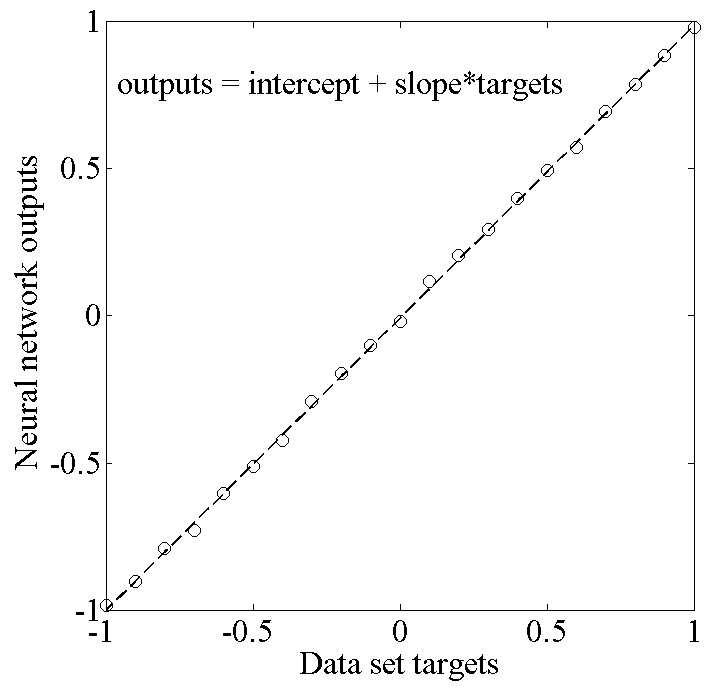
\includegraphics[width=0.6\textwidth]{function_regression/linear_regression_analysis.png}
\caption{Linear regression analysis.}\label{LinearRegressionAnalysis}
\end{center}
\end{figure}

